\chapter{スクレイピングを学ぼう}
\section{今回の授業}
\subsection*{目標 : }
\subsubsection*{ウェブページから\ruby{欲}{ほ}しい\ruby{情報}{じょうほう}を取り出す(スクレイピング)について学ぼう}
\subsection*{注意点}
\begin{itemize}
\item
授業の合間のきゅうけいでは、遠くのものをながめたりして目を休めましょう
\item 水分ほきゅうはこまめにしましょう
\item
先生が説明中は先生の話を聞きましょう
\item
わからないことがあったらTAの先生方にすぐ聞きましょう
\end{itemize}
\subsection*{教科書について}
\begin{itemize}
\item
教科書には例題、それに\ruby{似}{に}た問題があります

\begin{itemize}
\item
まずは、例題をよく読みながら試してみましょう
\item そのあと問題を\ruby{解}{と}きましょう
\end{itemize}
\item
例題、問題をクリアしたらシールラリーカードにシールを\ruby{貼}{は}りましょう
\item
授業中にすべての例題、問題をクリアできたらTAの先生にシールラリーカードを見せて、Complete(コンプリート)シールを\ruby{貰}{もら}いましょう
\item
授業中に終わらなかった例題、問題は宿題になるので、できるだけ授業中に終わらせましょう
\item
授業中にわからないところがあったらすぐにTAの先生に聞きましょう
\item
家でわからないことがあったら、すぐに\ruby{質問}{しつもん}フォームから質問しましょう。
\end{itemize}

\subsection*{教材を自分のフォルダに置こう}
まずは、今回利用する教材をコピーしましょう。
これまでと同じように、/usr/local/share/ome という場所にあるフォルダ 08をコピーして、/home/ユーザー名 に貼り付けてください。

やり方を忘れてしまった人は、「第1回 4.1 例題1-18 教材をじぶんのフォルダに置こう」 を参考にしてみてください。

\bigskip


\bigskip

\clearpage
\refstepcounter{PagePtr}\label{P:intro}
\section{ウェブページから情報を取り出す(\ruby{準備}{じゅんび})}
ウェブページから自分の必要な情報のみ取り出す方法を学びます。
まずはプログラムから自動で情報を取り出すのではなく、スクレイピングの仕組みを理解するために、一つずつ手動で行います。



\bigskip

{\bfseries\color[rgb]{1.0,0.2,0.2}
※ \ruby{講義}{こうぎ}では友達のIPアドレスやwebページを使っていますが、\ruby{個人}{こじん}で勉強する時は自分の }

{\bfseries\color[rgb]{1.0,0.2,0.2}
    IPアドレスやwebページを使って例題や問題を行ってください。}

手順
\begin{enumerate}

	\item
グループの席を円と考えましょう。左となりの友達を\ruby{確認}{かくにん}します


\bigskip



\begin{center}
  % Unhandled or unsupported graphics:
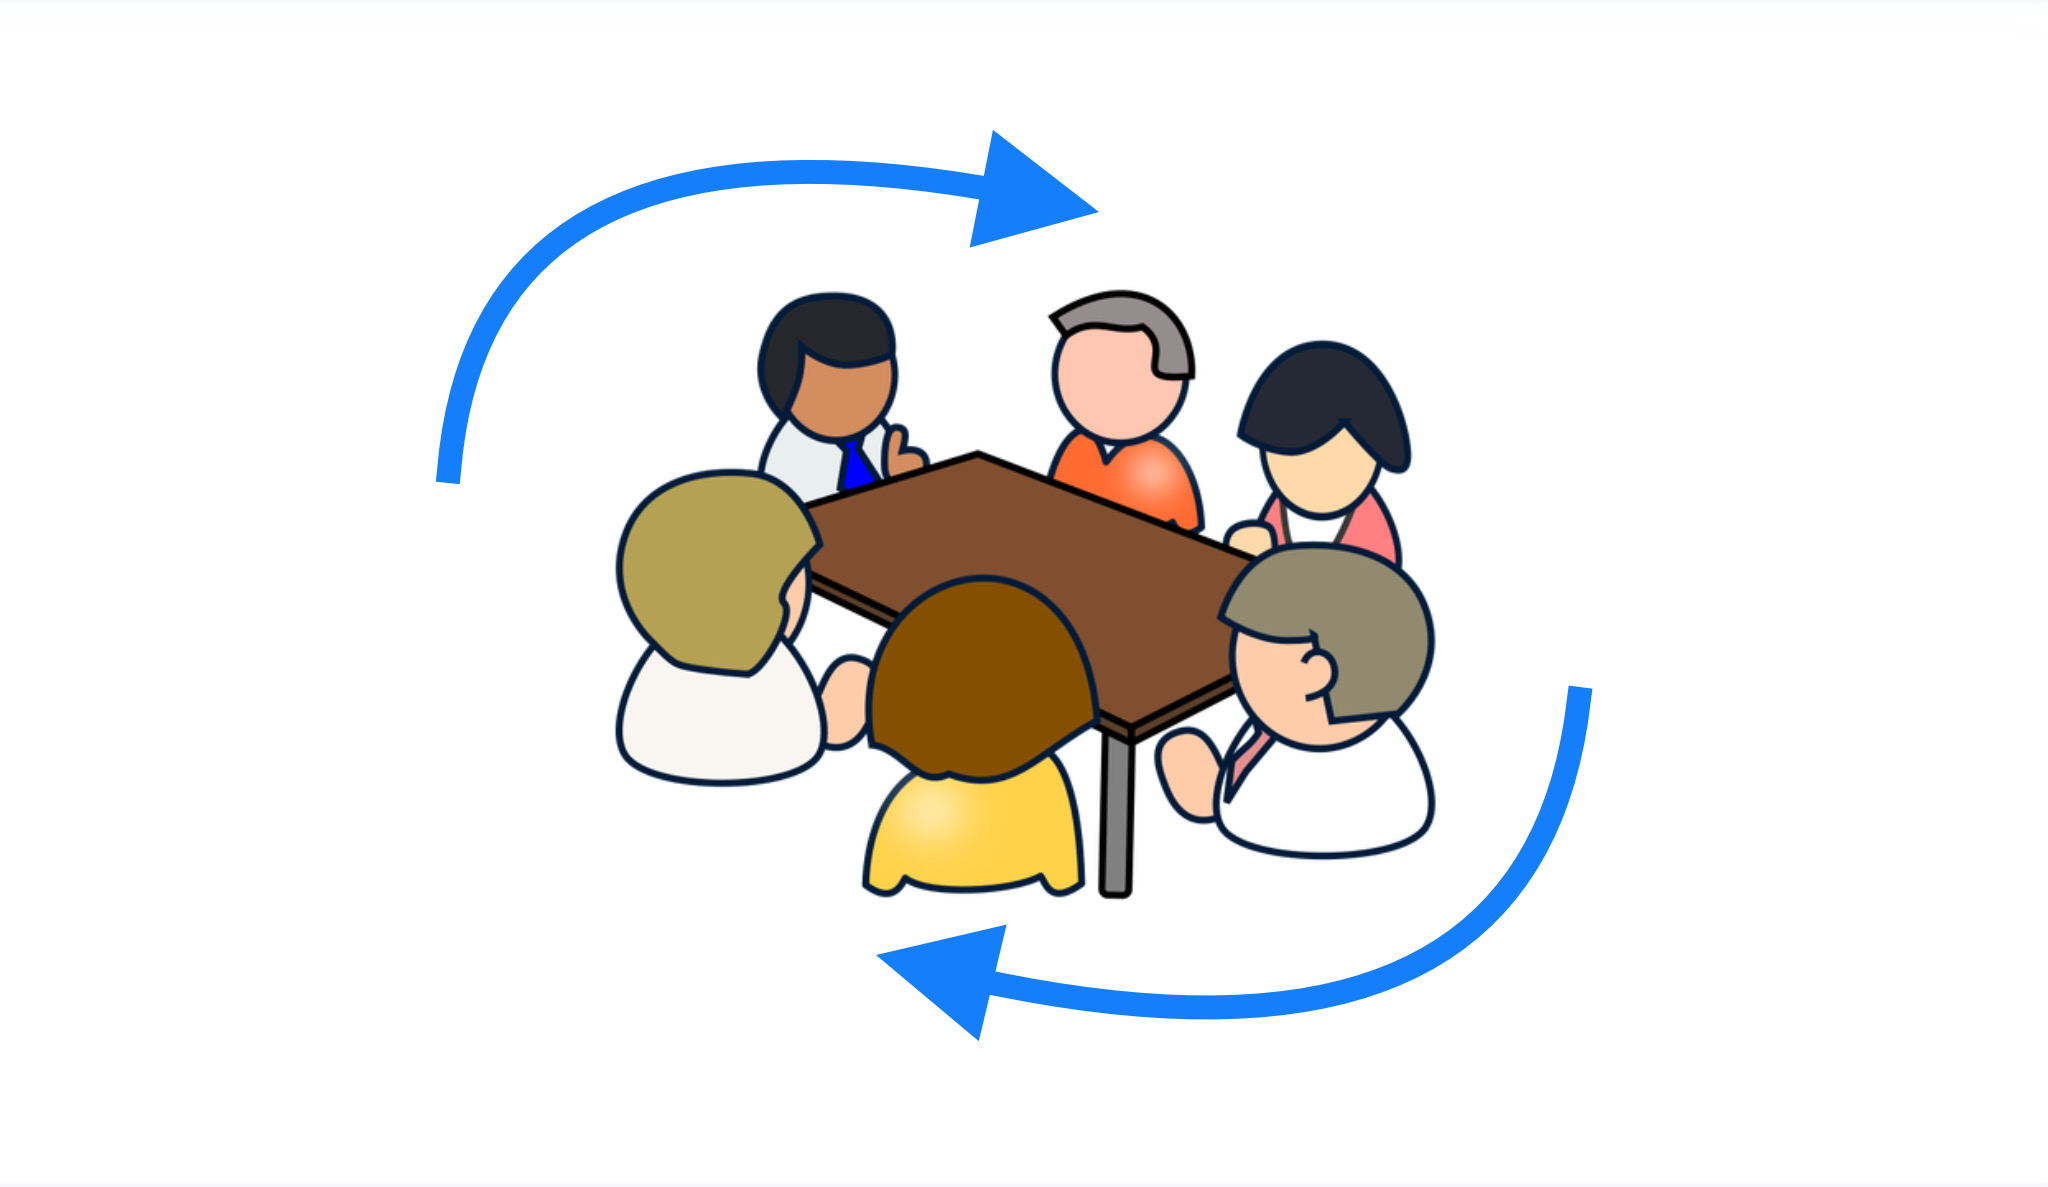
\includegraphics[width=10.174cm]{./text08-img/textbook-img001.jpg}

\end{center}

\bigskip


\bigskip


\bigskip



\item
左となりの人の\ruby{自己紹介}{じこしょうかい}ページをダウンロードします

\item
ダウンロードしたページを調べてみましょう。
\end{enumerate}

練習として、左となりの友達のウェブページから情報を取り出します。

そのための準備をしましょう。

第1回目の授業でみさなんが作成した自己紹介ページとその画像のファイルを第8回のフォルダにコピーしましょう。

やり方を忘れてしまった人は、「第7回 2-1 例題7-4 HTMLの復習」 を参考にしてみてください。

\textbf{cp \ {\textasciitilde}/01/self\_intro.html \ \ {\textasciitilde}/08/www/index.html}



\begin{center}
  % Unhandled or unsupported graphics:
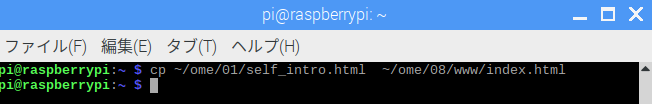
\includegraphics[width=\textwidth]{./text08-img/textbook-img002.png}

\end{center}
\clearpage
そのあと、ウェブサーバーを立ち上げます。

ウェブサーバの使い方については「付録 webserver.pyの使い方」を確認してください。

\textbf{cd \ {\textasciitilde}/08/www}

\textbf{./webserver.py}



\begin{center}
  % Unhandled or unsupported graphics:
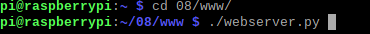
\includegraphics[width=\textwidth]{./text08-img/textbook-img003.png}

\end{center}
ウェブサーバーは3000番ポートで動いています。(ポートについては、「7回目の教科書
ポートについて」を確認してください)%
%7会のリファレンス
%koyaman
%September 23, 2019 10:21 PM


ウェブサーバにアクセスする\ruby{際}{さい}は、IPアドレスとともに3000番のポートを指定する必要があります。

このターミナルは\ruby{閉}{と}じずに、もう一つターミナルを開いてください。

\textbf{hostname -I}

を実行して右となりの人にIPアドレスを教えてください。

\begin{center}
  % Unhandled or unsupported graphics:
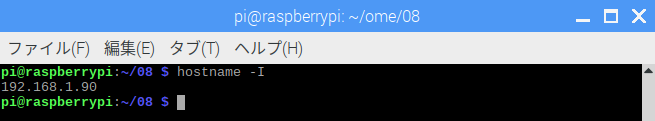
\includegraphics[width=\textwidth]{./text08-img/textbook-img004.png}

\end{center}
\clearpage\subsection*{IPアドレスメモらん}
IPアドレスをメモするのに使ってください。

% \begin{center}
% \tablefirsthead{}
% \tablehead{}
% \tabletail{}
% \tablelasttail{}
% \begin{supertabular}{|m{5.4690003cm}|m{5.4690003cm}|m{5.4690003cm}|}
% \hline
% 日付

% 例: 9/29 &
% 名前

% 例: あずまくん &
% IPアドレス:ポート

% 例: 192.168.1.100:3000\\\hline
% ~

% ~

% ~

% ~
%  &
% ~
%  &
% ~
% \\\hline
% ~

% ~

% ~

% ~
%  &
% ~
%  &
% ~
% \\\hline
% ~

% ~

% ~

% ~
%  &
% ~
%  &
% ~
% \\\hline
% ~

% ~

% ~

% ~
%  &
% ~
%  &
% ~
% \\\hline
% ~

% ~

% ~

% ~
%  &
% ~
%  &
% ~
% \\\hline
% \end{supertabular}
% \end{center}


\begin{table}[htbp]
    \centering
    % \caption{文字タイプ表}
    \begin{tabular}{|l|l|l|}
        \hline
        \begin{tabular}{l}
            日付\\
            例:9/29
        \end{tabular}
        & 
        \begin{tabular}{l}
            名前\\
            例:あずまくん
        \end{tabular}
        & 
        \begin{tabular}{l}
            IPアドレス:ポート\\
            例:192.168.1.100:3000
        \end{tabular}

		  \\\hline
      \begin{tabular}{l}
                          \\
                          \\
                          \\
                          \\
      \end{tabular}
      & 
      \begin{tabular}{l}
                          \\
                          \\
                          \\
                          \\
      \end{tabular}
      & 
      \begin{tabular}{l}
                          \\
                          \\
                          \\
                          \\
      \end{tabular}
        
      \\\hline
      \begin{tabular}{l}
                          \\
                          \\
                          \\
                          \\
      \end{tabular}
      & 
      \begin{tabular}{l}
                          \\
                          \\
                          \\
                          \\
      \end{tabular}
      & 
      \begin{tabular}{l}
                          \\
                          \\
                          \\
                          \\
      \end{tabular}
        
      \\\hline
      \begin{tabular}{l}
                          \\
                          \\
                          \\
                          \\
      \end{tabular}
      & 
      \begin{tabular}{l}
                          \\
                          \\
                          \\
                          \\
      \end{tabular}
      & 
      \begin{tabular}{l}
                          \\
                          \\
                          \\
                          \\
      \end{tabular}
        
      \\\hline
      \begin{tabular}{l}
                          \\
                          \\
                          \\
                          \\
      \end{tabular}
      & 
      \begin{tabular}{l}
                          \\
                          \\
                          \\
                          \\
      \end{tabular}
      & 
      \begin{tabular}{l}
                          \\
                          \\
                          \\
                          \\
      \end{tabular}
        
      \\\hline
      \begin{tabular}{l}
                          \\
                          \\
                          \\
                          \\
      \end{tabular}
      & 
      \begin{tabular}{l}
                          \\
                          \\
                          \\
                          \\
      \end{tabular}
      & 
      \begin{tabular}{l}
                          \\
                          \\
                          \\
                          \\
      \end{tabular}
        
      \\\hline
        
    \end{tabular}
\end{table}
\bigskip

\refstepcounter{Exercise}
\clearpage\section{\theExercise コマンドラインからウェブページをダウンロードする}
\addtocounter{Exercise}{-1}\refstepcounter{Exercise}\label{E:CURL}
インターネットから情報を取ってくるときに使用するツールは
curl (カール)と言います。 curl
はデータを送ったり受け取ったりするときに使います。

左となりの友達のウェブページを取得してみましょう。

\ruby{保存}{ほぞん}するファイル名はローマ字で”友達の名前.html”にしましょう。

例 : koyama.html

例題ではfriend.htmlとして保存しています。

ターミナルを開いてください。

\textbf{cd \ {\textasciitilde}/08}

curl “左となりの友達のIPアドレス”:3000/index.html -o
friend.html

\ \ 例 :
IPアドレスが192.168.1.90の友達のIPアドレス

\ \ → curl 192.168.1.90:3000/index.html -o friend.html

を実行します。

\begin{center}
  % Unhandled or unsupported graphics:
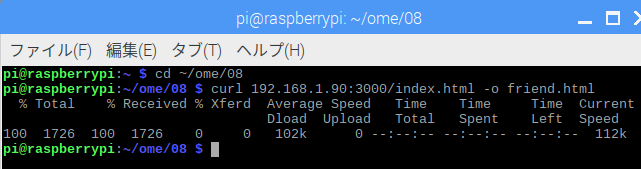
\includegraphics[width=\textwidth]{./text08-img/textbook-img005.png}

\end{center}

\bigskip

HTMLファイルをダウンロードしてfriend.htmlとして保存しています。



% \begin{center}
% \begin{boxedminipage}{17.228cm}
% \section*{コラム
% curlコマンドのオプション(\ruby{機能}{きのう})}

% \bigskip

% curlコマンドを何もオプションをつけないで実行すると、ターミナルにダウンロードした情報を\ruby{表示}{ひょうじ}します。コマンドに”-o”オプションをつけることで、ターミナルに表示する代わりに、ファイルに保存することができます。

% “-o
% “の後に保存するファイル名を指定します。

% 	\textbf{curl URL -o ファイル名}
% \end{boxedminipage}
% \end{center}

\begin{table}[htbp]
    \centering
    % \caption{文字タイプ表}
    \begin{tabular}{|l|}
        \hline
        \begin{tabular}{l}
            % \section*{コラム curlコマンドのオプション(機能)}
            コラム curlコマンドのオプション(\ruby{機能}{きのう})\\
            \\
            curlコマンドを何もオプションをつけないで実行すると、ターミナルにダウンロードした情報\\
            を表示します。コマンドに”-o”オプションをつけることで、ターミナルに\ruby{表示}{ひょうじ}する代わりに、\\
            ファイルに保存することができます。\\
            "-o"の後に保存するファイル名を指定します。\\
            \textbf{curl URL -o ファイル名}
            \\\hline
        \end{tabular}
        
    \end{tabular}
\end{table}


\clearpage
これでダウンロードができました。実際にダウンロードしたファイルが左となりの友達のウェブページかどうかmousepadで開いて確認してみましょう。



\begin{center}
  % Unhandled or unsupported graphics:
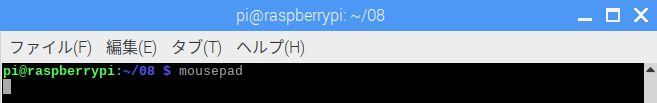
\includegraphics[width=\textwidth]{./text08-img/textbook-img006.png}

\end{center}
ファイル(F) → 開く(O)..

をクリックして\textbf{{\textasciitilde}/08/friend.html}

を開きます。自己紹介のらんにある名前を\ruby{探}{さが}して確認してみよう。



\begin{center}
  % Unhandled or unsupported graphics:
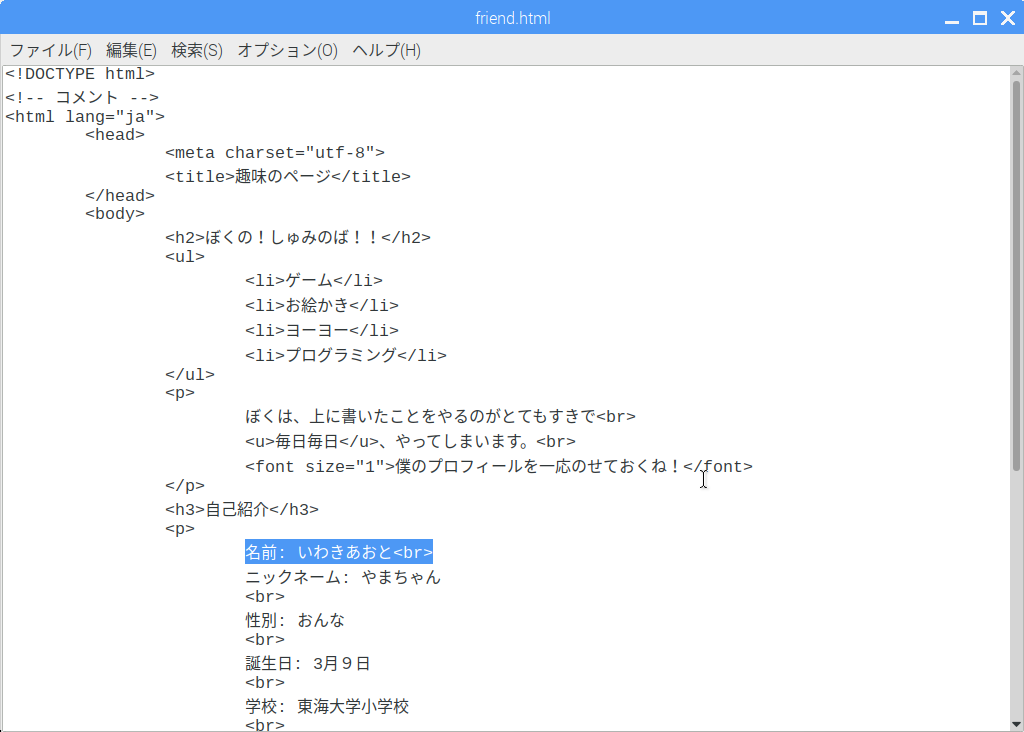
\includegraphics[width=\textwidth]{./text08-img/textbook-img007.png}

\end{center}

\bigskip

”いわきあおと”のウェブページのHTMLファイルがダウンロードできていることが確認できました。

次はダウンロードしたHTMLファイルから情報を取り出してみよう。
\refstepcounter{Question}
\clearpage\subsection*{\theQuestion\label{Q:CURL}}
\begin{itemize}
\item curl
を使って、グループの友達全員のウェブページを保存しよう。
\end{itemize}
\ \ \ \ Hint :
ローマ字を使って”友達の名前.html”にしておこう

\ \ \ \ (例: koyama.html)

\refstepcounter{Question}
\subsection*{\theQuestion\label{Q:HTML}}
\begin{itemize}
\item
mousepadを使ってダウンロードしたHTMLファイルを開いて友達の名前を確認してみよう
\end{itemize}
\ \ \ \ Hint :
ダウンロードしたファイルをmousepadで見てみよう

\refstepcounter{Exercise}
\clearpage\section{\theExercise ダウンロードしたページを調べてみましょう}
\addtocounter{Exercise}{-1}\refstepcounter{Exercise}\label{E:HTML}
考え方


\ref*{E:CURL}で、友達のウェブページのHTMLをダウンロードしました。次はほしい情報を取り出します。ここでは、テキストエディタで\ruby{検索}{けんさく}をして、ほしい情報を探し\ruby{抜}{ぬ}き出します。

コマンドラインを開いて

\textbf{cd \ {\textasciitilde}/08/}

mousepad



\begin{center}
  % Unhandled or unsupported graphics:
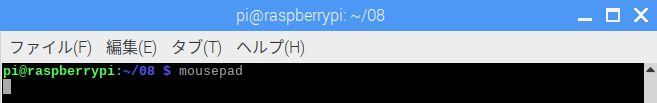
\includegraphics[width=\textwidth]{./text08-img/textbook-img006.png}

\end{center}
を実行してください。

テキストエディタが開きます。

ファイル(F) → 開く(O)..

をクリックして\textbf{{\textasciitilde}/08/friend.html}



\begin{center}
  % Unhandled or unsupported graphics:
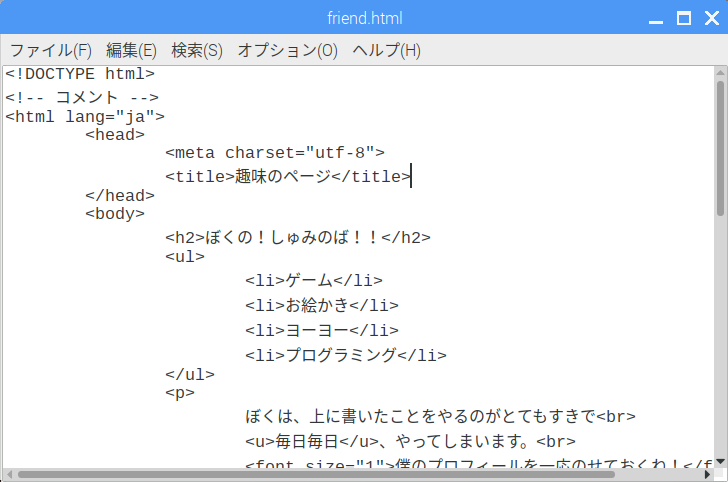
\includegraphics[width=\textwidth]{./text08-img/textbook-img008.png}

\end{center}


\bigskip


\bigskip

\clearpage
友達のウェブページのタイトルをテキストエディタで探してみましょう。

タイトルはブラウザのタブに表示されるもので{\textless}title{\textgreater}{\textless}/title{\textgreater}タグで作ったことを思い出しましょう。



\begin{center}
  % Unhandled or unsupported graphics:
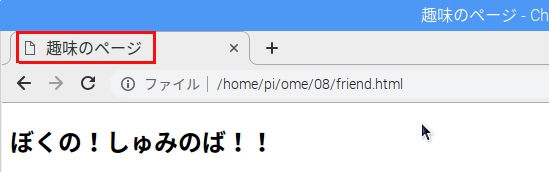
\includegraphics[width=\textwidth]{./text08-img/textbook-img009.png}

\end{center}

\bigskip

テキストエディタで{\textless}title{\textgreater}{\textless}/title{\textgreater}タグを探してみましょう。

検索-{\textgreater}検索(F)..をクリックします。

\begin{center}
  % Unhandled or unsupported graphics:
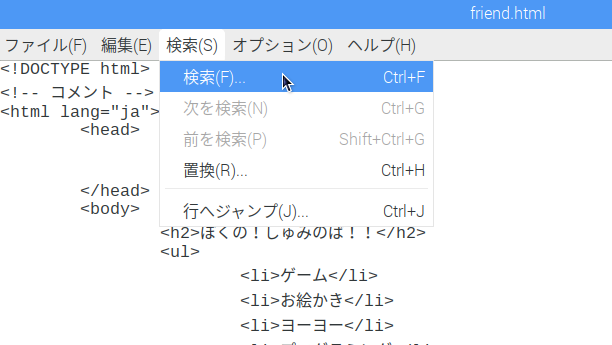
\includegraphics[width=\textwidth]{./text08-img/textbook-img010.png}

\end{center}
\clearpage
検索する文字列には検索したい文字列を入れます。この例では{\textless}title{\textgreater}{\textless}/title{\textgreater}を探したいので、

{\textless}title{\textgreater}と入れます。検索をクリックします。

{\bfseries
注意 :
{\textless}title{\textgreater}は半角文字です。入力モードが半角になっているか確認してください。(\ruby{詳}{くわ}しくは例題1-4を見てください)}



\begin{center}
  % Unhandled or unsupported graphics:

\includegraphics[width=\textwidth]{./text08-img/textbook-img012.png}

\end{center}
見つかった結果を色を変えて表示してくれます。これで、ウェブページからほしい情報を見つけることができました。


\bigskip

毎回手動で友達のウェブページをダウンロードして、検索して探すのは大変です。次はプログラムから自動で行う方法を学びましょう。
\refstepcounter{Exercise}
\clearpage\section{\theExercise HSPから情報を取り出す}
\addtocounter{Exercise}{-1}\refstepcounter{Exercise}\label{E:SCRAPING}
考え方

前の例題でやったように、毎回手動で友達のウェブページをダウンロードして、テキストエディタを使って検索するのは大変です。
また、ウェブページが\ruby{更新}{こうしん}されたら、同じ手順を\ruby{繰}{く}り返して情報を取り直さないといけません。
そこで、今回はこの手順をHSPのプログラムで自動で行う方法を学びます。

友達のウェブページからウェブページのタイトルを取り出してみよう。

まずはプログラムを動かしてみましょう。

ターミナルからHSPスクリプトエディタを開きます。

ターミナルを開いて、

hsed を実行してください



\begin{center}
  % Unhandled or unsupported graphics:
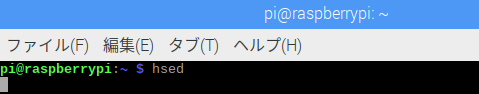
\includegraphics[width=\textwidth]{./text08-img/textbook-img013.png}

\end{center}

\clearpage

ファイル→開く から\\
\textbf{{\textasciitilde}/08/title.hsp}

を開いてください



\begin{center}
  % Unhandled or unsupported graphics:
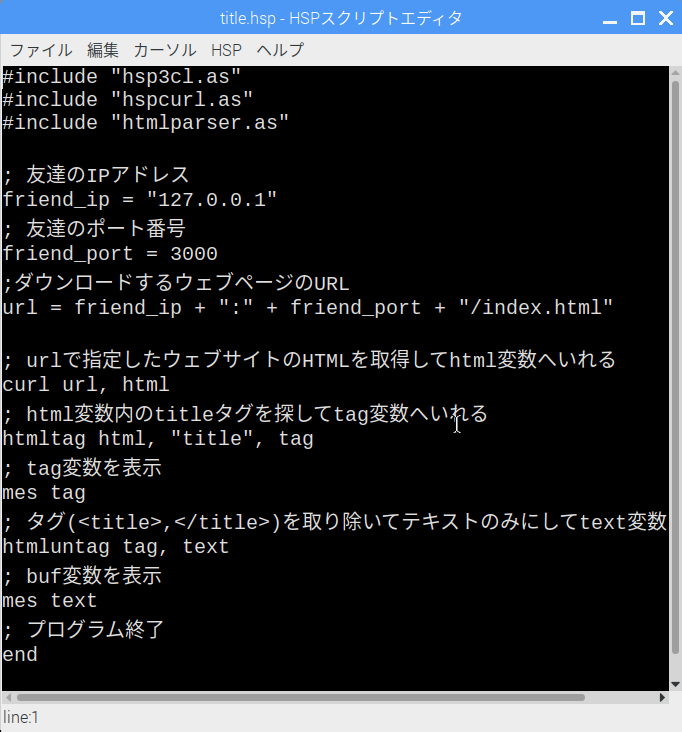
\includegraphics[width=11.472cm]{./text08-img/textbook-img014.png}

\end{center}

\bigskip


\bigskip

\clearpage
6行目のfriend\_ip =
“127.0.0.1”を友達のIPアドレスに変えましょう。


例 : 友達のIPアドレスが”192.168.1.90”の場合

\ \ → friend\_ip = “192.168.1.90”

F5を\ruby{押}{お}して実行してみましょう。
実行結果はhsedを実行したターミナルに表示されます。



\begin{center}
  % Unhandled or unsupported graphics:
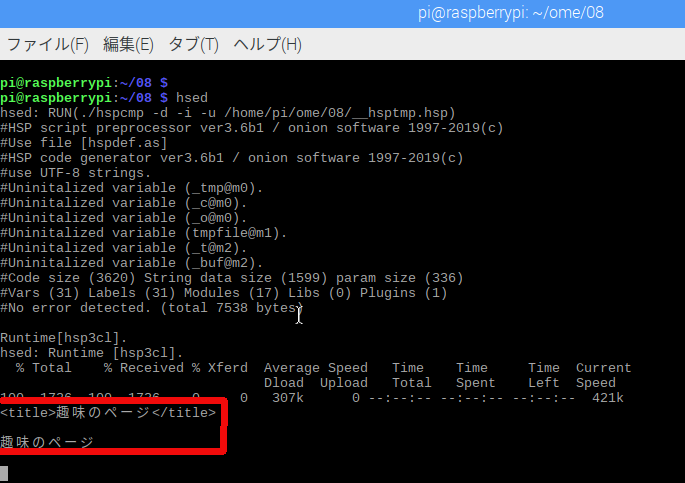
\includegraphics[width=0.9\textwidth]{./text08-img/textbook-img015.png}

\end{center}


\bigskip


\bigskip

このように手動でHTMLファイルをダウンロードして、テキストエディタで開いて、タイトルを検索して情報を取り出したのをプログラムで行うことができます。
次にプログラムの中身を見てみましょう。

\clearpage
プログラム解説



% \begin{center}
% \begin{boxedminipage}{16.053cm}
% \setlength{\itemsep}{0cm} % 項目間
% \setlength{\parskip}{0cm} % 項目間
% \begin{enumerate}
% \baselineskip 10pt
% \setlength{\itemsep}{0cm} % 項目間
% \item \#include {\textquotedbl}hsp3cl.as{\textquotedbl}
% \item \#include {\textquotedbl}hspcurl.as{\textquotedbl}
% \item \#include {\textquotedbl}htmlparser.as{\textquotedbl}
% \item
% \item ; 友達のIPアドレス
% \item friend\_ip = {\textquotedbl}127.0.0.1{\textquotedbl}
% \item ; 友達のポート番号
% \item friend\_port = 3000
% \item ;ダウンロードするウェブページのURL
% \item url = friend\_ip + {\textquotedbl}:{\textquotedbl} + friend\_port + {\textquotedbl}/index.html{\textquotedbl}
% \item
% \item ;
% urlで指定したウェブページのHTMLを取得してhtml変数へいれる
% \item curl url, html
% \item ;
% html変数内のtitleタグを探してtag変数へいれる
% \item htmltag html, {\textquotedbl}title{\textquotedbl}, tag
% \item ; tag変数を表示
% \item mes tag
% \item ;
% タグ({\textless}title{\textgreater},{\textless}/title{\textgreater})を取り\ruby{除}{のぞ}いてテキストのみにしてtext変数に入れる
% \item htmluntag tag, text
% \item ; buf変数を表示
% \item mes text
% \item ; プログラム\ruby{終了}{しゅうりょう}
% \item end
% \end{enumerate}
% \end{boxedminipage}
% \end{center}




\begin{table}[htbp]
    \centering
    % \caption{文字タイプ表}
    \begin{tabular}{|l|}
        \hline
        
        1. \#include {\textquotedbl}hsp3cl.as{\textquotedbl}\\ 
        2. \#include {\textquotedbl}hsp3cl.as{\textquotedbl}\\
        3. \#include {\textquotedbl}hspcurl.as{\textquotedbl}\\
        4. \#include {\textquotedbl}htmlparser.as{\textquotedbl}\\
        5.\\
        6. ; 友達のIPアドレス\\
        7. friend\_ip = {\textquotedbl}127.0.0.1{\textquotedbl}\\
        8. ; 友達のポート番号 \\
        9. friend\_port = 3000\\
        10. ;ダウンロードするウェブページのURL\\
        11. url = friend\_ip + {\textquotedbl}:{\textquotedbl} + friend\_port + {\textquotedbl}/index.html{\textquotedbl}\\
        12.\\
        13. ;urlで指定したウェブページのHTMLを取得してhtml変数へいれる\\
        14. curl url, html\\
        15. ;html変数内のtitleタグを探してtag変数へいれる\\
        16. htmltag html, {\textquotedbl}title{\textquotedbl}, tag\\
        17. ; tag変数を表示\\
        18. mes tag\\
        19. ;タグ({\textless}title{\textgreater},{\textless}/title{\textgreater})を取り除いてテキストのみにしてtext変数に入れる\\
        20. htmluntag tag, text\\
        21. ; buf変数を表示  \\
        22. mes text\\
        23. ; プログラム終了\\
        24. end\\
        
        \hline
    \end{tabular}
\end{table}




\bigskip



\bigskip

6行目のfriend\_ip変数にはウェブページをダウンロードする友達のIPアドレスを入れます。

自分のウェブページをダウンロードしたい場合は、”127.0.0.1”を指定します。


\bigskip

8行目のfriend\_port変数にはウェブサーバが動いているポートを指定します。
3000番でウェブサーバが動いているので、3000にしておきます。


\bigskip

10行目のurl変数は、ダウンロードするウェブページを表すURLを指定します。

この例題プログラムでは、127.0.0.1:3000/index.htmlのような形になっています。


\bigskip

13行目では、実際にウェブページをダウンロードしてhtml変数へいれています。

curl url, html

はurl変数で指定されているウェブページをダウンロードしてファイルの中身をhtml変数へ読み\ruby{込}{こ}んでいます。


\bigskip

\clearpage
15行目の

htmltag html, “title”, tag

では、html変数にあるHTMLから{\textless}title{\textgreater}{\textless}/title{\textgreater}タグを探して、結果をtag変数へいれています。


\bigskip

% \begin{center}
% \tablefirsthead{}
% \tablehead{}
% \tabletail{}
% \tablelasttail{}
% \begin{supertabular}{|m{16.806cm}|}
% \hline
% htmltag命令の使い方

% \textbf{htmltag} \textbf{もとの変数, “タグ”,
% 結果を入れる変数}

% 例: htmltag src, “title”, dest

%  src変数からtitleタグを探して、dest変数へ結果を入れる。\\\hline
% \end{supertabular}
% \end{center}




\begin{table}[htbp]
    \centering
    % \caption{文字タイプ表}
    \begin{tabular}{|l|}
        \hline
        
        htmltag命令の使い方\\

        \textbf{htmltag} \textbf{もとの変数, “タグ”,結果を入れる変数}\\
        例: htmltag src, “title”, dest\\
        src変数からtitleタグを探して、dest変数へ結果を入れる。
        
        \\\hline
    \end{tabular}
\end{table}



\bigskip

17行目では、titleタグの検索結果を表示しています。

表示結果では、{\textless}title{\textgreater}\ruby{趣味}{しゅみ}のページ{\textless}/title{\textgreater}となっています。

実際に欲しい情報は{\textless}title{\textgreater}{\textless}/title{\textgreater}の間にある文字列つまりこの例では、”趣味のページ”です。



\begin{center}
  % Unhandled or unsupported graphics:
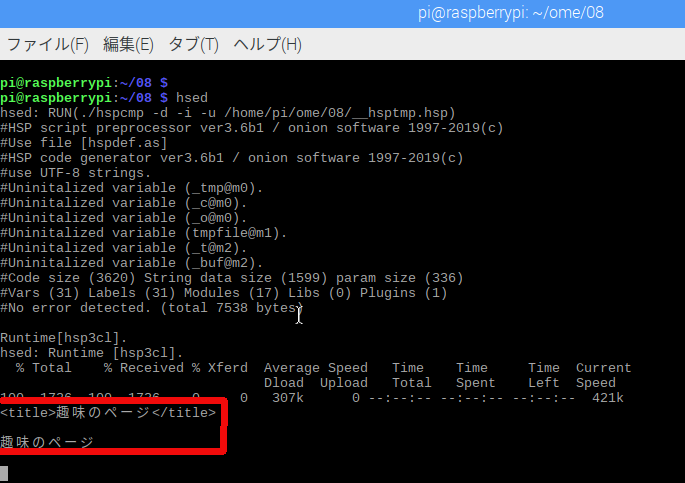
\includegraphics[width=0.9\textwidth]{./text08-img/textbook-img015.png}

\end{center}


\bigskip


\bigskip

\clearpage
19行目の

htmluntag tag, text

では、tag変数にあるタグをすべて取り外して、間にあるテキストのみにして、text変数へいれています。


\bigskip

% \begin{center}
% \tablefirsthead{}
% \tablehead{}
% \tabletail{}
% \tablelasttail{}
% \begin{supertabular}{|m{16.806cm}|}
% \hline
% htmluntag命令の使い方

% {\bfseries htmluntag もとの変数, 結果を入れる変数}

% 例: htmluntag src, dest

% src変数のタグを取り外してタグの間にあるテキストだけにしてdest変数へ結果を入れる。\\\hline
% \end{supertabular}
% \end{center}


\begin{table}[htbp]
    \centering
    % \caption{文字タイプ表}
    \begin{tabular}{|l|}
        \hline
        
        htmluntag命令の使い方\\

        {\bfseries htmluntag もとの変数, 結果を入れる変数}\\

        例: htmluntag src, dest\\

        src変数のタグを取り外してタグの間にあるテキストだけにしてdest変数へ結果を入れる。
        \\\hline
    \end{tabular}
\end{table}


\bigskip

21行目では、{\textless}title{\textgreater}{\textless}/title{\textgreater}タグを取り外した結果を表示させています。

タグを取り外したので、{\textless}title{\textgreater}趣味のページ{\textless}/title{\textgreater}の間の文字列である”趣味のページ”のみ表示されています。
ほしいテキストのみを取り出すことができました。



\begin{center}
  % Unhandled or unsupported graphics:
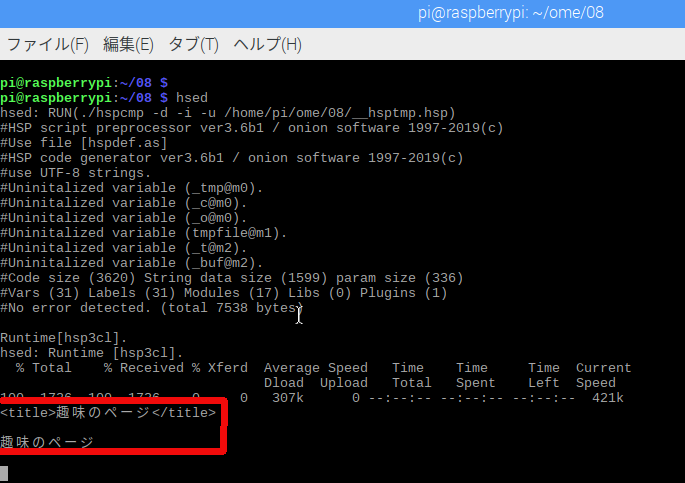
\includegraphics[width=0.9\textwidth]{./text08-img/textbook-img015.png}

\end{center}

\bigskip


\bigskip

このようにさっきターミナルやテキストエディタで\ruby{頑張}{がんば}って手動で行った動作をプログラムで行うことができました。
プログラムから情報を取り出すことができると、取り出した情報を使ってウェブページを作ったり、情報をもとにセンサーなどを\ruby{操作}{そうさ}できるようになります。
例えば、次の例で試すアメダスとよばれる\ruby{気象情報観測}{きしょうじょうほうかんそく}システムの観測情報(気温、\ruby{降水確率}{こうすいかくりつ})などの情報を取り出し、LEDなどのセンサーと組み合わせます。
\ruby{実現}{じつげん}したいアイディアがあったらメモをしておきましょう。

\refstepcounter{Question}
\clearpage\subsection*{\theQuestion\label{Q:title}}
\begin{itemize}
\item
残りのグループ内の友達のウェブページのタイトルを取り出してみよう
\end{itemize}
\ \ HINT:
firend\_ipでダウンロードしたい友達のIPアドレスを指定する

\ \ \ \ メモした友達のIPアドレスを使おう

\refstepcounter{Question}
\subsection*{\theQuestion\label{Q:mes}}
\begin{itemize}
\item 13行目 curl url, htmlの下の行にmes
htmlを追加して、実際にダウンロードされたHTMLを確認してみよう
\end{itemize}
\ \ HINT : 14行目にmes htmlを書く

\refstepcounter{Question}
\subsection*{\theQuestion\label{Q:ol}}
\begin{itemize}
\item 15行目のhtmltag html, “title”,
tagの”title”を”ol”に変更してみましょう
\end{itemize}
\ \ HINT: htmltag html, “ol”, tag

\ \ htmltag html, “title”,
tag命令はtag変数の中に、
”{\textless}title{\textgreater}...{\textless}/title{\textgreater}”
を探した結果を入れています。
”title”を”ol”に変えると“
{\textless}ol{\textgreater}...{\textless}/ol{\textgreater}”
タグを探して、結果を入れてくれます。


\refstepcounter{Question}
\subsection*{\theQuestion\label{Q:tag}}
\begin{itemize}
\item 15行目のhtmltag html, “title”,
tagの”title”を探したいタグへ変更しよう
\end{itemize}
\ \ HINT: pタグを探したい場合

\ \ \ \ \ htmltag html, “p”, tag

